
\chapter{Related Work}

\section{Emotion representation}
A still widely discussed research question in Emotion Recognition is the question about how to best represent emotions or how to model affect. \citet{Gunes:2011:EmotionRepresentationContinuous} state that current approaches stem from research in psychology, which distinguishes between three major approaches: \textbf{categorical, dimensional and appraisal-based.}
% According to research in psychology, three major approaches to affect modelling can be distinguished [1]: categorical, dimensional and appraisal-based approach. The categorical approach claims that there exist a small number of emotions that are basic, hard-wired in our brain and recognised universally (e.g., [2]). This theory on universality and interpretation of affective nonverbal expressions in terms of basic emotion categories has been the most commonly adopted approach in research on automatic measurement of human affect.
% \citep{Gunes:2011:EmotionRepresentationContinuous}
\newline\newline
The \textbf{categorical approach} classifies emotions into a small number of discrete categories which are universally recognised. Usually, these are comprised of six or seven categories, which include 'happy', 'sad', 'fear', 'anger', 'disgust', 'surprise' and sometimes also 'neutral' \citep{Hupont:2010:FacialEmotionsIn2DAffectiveSpace}. Even though there are many other ways to represent emotions, \citet{Salah:2018:VideoBasedER} argue, that this approach is still very relevant today, as its more natural for humans to interpret emotions in that way. This is supported by \citet{Gunes:2011:EmotionRepresentationContinuous} who say that the theory on universality, as well as the facility of interpretation has made this approach the most commonly adopted in research on automatic measurement of human affect.
\newline\newline
However, \citet{Gunes:2011:EmotionRepresentationContinuous} argues that this categorical approach is not able to capture the complexity of the affective state exhibited by people in a rather complex and subtle ways, like embarrassment.
% However, a number of researchers have shown that in everyday interactions people exhibit non-basic, subtle and rather complex affective states like thinking, embarrassment or depression. Such subtle and complex affective states can be expressed via dozens of anatomically possible facial and bodily expressions, audio or physiological signals. Therefore, a single label (or any small number of discrete classes) may not reflect the complexity of the affective state conveyed by such rich sources of information
% \citep{Gunes:2011:EmotionRepresentationContinuous}
\newline\newline
%The most widely used dimensional model is a circular configuration called Circumplex of Affect introduced by Russell [3]. This model is based on the hypothesis that each basic emotion represents a bipolar entity being a part of the same emotional continuum. The proposed polars are arousal (relaxed vs. aroused) and valence (pleasant vs. unpleasant)
% \citep{Gunes:2011:EmotionRepresentationContinuous}
A widely used \textbf{dimensional approach} called 'Continuous Affective Space' was proposed by \citet{Hupont:2010:FacialEmotionsIn2DAffectiveSpace} and consists of representing emotions as a point in a two-dimensional plane instead of discrete categories. Thus, they represent an emotion as a combination of two values, valence and arousal. While valence indicates how positive or negative an emotion is, arousal indicates how calming or exciting an emotion is. \citet{Hupont:2010:FacialEmotionsIn2DAffectiveSpace} claim that this approach allows them to to capture more information by considering intermediate emotional states.
% Hupont, Cerezo, and Baldassarri(2010): Continous Affective Space, mapping emotions into a 2D space allowing them to consider intermediate emotional states (intermediate emotional state = in-between emotions, gradients of emotions e.g., anxiety to fear, horror to disgust [presumably]). This study allowed for the representation of emotions as a point in a plane, instead of mere items in a categorical list.
% Valence (whether emotion is + or -), arousal (strength of the emotion of expression)
% \citep{Hupont:2010:FacialEmotionsIn2DAffectiveSpace}
\newline\newline
However, \citet{Salah:2018:VideoBasedER} object that a complex emotion can be reduced to a point in a valence-arousal region. She uses 'love' to exemplify that an emotion can be attributed with a positive or negative value depending on the context. As we would usually identify 'love' with a positive valence, a concerned expression of a mother looking at her sick child could be mapped to a negative valence. Therefore, \citet{Salah:2018:VideoBasedER} argue that there is still a need for mapping such points to a semantic space, so that humans can properly interpret the emotion.
% However, categorical and discrete approaches that go beyond the six (or seven, if we include “contempt”) basic expressions are still very relevant, as their interpretation is more natural for humans. Also, it is difficult to reduce a complex emotion to a point or region in the valence-arousal space. For instance, we can claim that “love” is a positive emotion, and has a positive valence, but this is not always the case. Consider the loving, concerned expression of a mother, looking at her sick child, and this becomes obvious. Subsequently, a given image or video can be annotated in the continuous space, but there is still a need for mapping such points to a semantic space, where it can be properly interpreted 
% \citep{Salah:2018:VideoBasedER}
\newline\newline
A further \textbf{dimensional approach} is built upon the previously described approaches and argue that even the two dimensional affective space with its valence and arousal is insufficient to represent the variety of emotions accurately. There exist different approaches, like the Pleasure, Arousal and Dominance (PAD) approach \citep{Gunes:2011:EmotionRepresentationContinuous} and the Valence, Arousal and Dominance (VAD) approach \citep{Verma:2017:3D-VAD}
% Another well-accepted and commonly used dimensional description is the 3D emotional space of pleasure – displeasure, arousal – nonarousal and dominance – submissiveness [4], at times referred to as the PAD emotion space [6] or as emotional primitives [7]
% \citep{Gunes:2011:EmotionRepresentationContinuous}
% The valence-arousal model is insufficient to represent emotions accurately. Thus, they introduce a 3D model, called Valence-Arousal-Dominance.
% \citep{Verma:2017:3D-VAD}
\newline\newline
\citet{Gunes:2011:EmotionRepresentationContinuous} points out that a major challenge for utilizing affective data is it's annotation process, as there exists no general annotation scheme agreed upon by all researchers. Therefore, it cannot be excluded, that the annotations possess a personal bias according to the human annotator's personal context and cultural background. Developing such an annotation scheme would need to be unambiguous and facilitate inter-observer agreement.
% A major challenge in affective data annotation is the fact that there is no coding scheme that is agreed upon and used by all researchers in the field that can accommodate all possible communicative cues and modalities. Development of an easy to use, unambiguous and intuitive annotation scheme that is able to incorporate inter-observer agreement levels will indeed ease the heavy burden of the annotation task. Obtaining high inter-observer agreement is another challenge in affect data annotation, especially when (continuous) dimensional approach is adopted.
% \citep{Gunes:2011:EmotionRepresentationContinuous}
\newline\newline
The \textbf{appraisal-based approach} is still considered by \citep{Gunes:2011:EmotionRepresentationContinuous} as an open research question for automatic measurement of affect. The approach consists in generating emotions through continuous subjective evaluation of the subject's internal state and the state of the outside world.
% In the appraisal-based approach emotions are generated through continuous, recursive subjective evaluation of both our own internal state and the state of the outside world (relevant concerns/needs) [1], [5], [8], [10]. Despite pioneering efforts of Scherer and colleagues (e.g., [11]), how to use the appraisal-based approach for automatic measurement of affect is an open research question as this approach requires complex, multicomponential and sophisticated measurements of change.
% \citep{Gunes:2011:EmotionRepresentationContinuous}


%%%%%%%%%%%%%%%%%%%%%%%%%%%%%%%%%%%%%%%%%%%%%%%%%%%%%%%%%%%%%%%%%%

\section{Emotion Recognition}
\begin{quote}
    Emotion recognition refers in psychology to the attribution of emotional states based on the observation of visual and auditory nonverbal cues. \citep{Baenziger:2014:MeasuringERAbility}
\end{quote}
In Computer Science, however, it often seems as if researchers directly equate facial expressions with peoples emotions. \citet{Barrett:2019:EmotionalFromFacialMovements} claim that based upon a review of psychological research, the belief of reliably corresponding facial expressions with emotions is unfounded. This is especially true for the categorical approach of emotion representation, as it favors human interpretability over precision. Therefore, it just assumes that only six or seven basic emotions exist which can be classified by the observation of visual and auditory nonverbal cues.
\newline\newline
Nevertheless, it has to be pointed out, that even this Master thesis, by only looking at facial expressions and by utilizing the AFEW-VA dataset with its annotations, has a inherent assumption that facial expressions correspond to a person's emotions.\newline
This raises the following question: How much of a person's facial expression actually corresponds to the real emotion?
\newline\newline
\citet{Barrett:2019:EmotionalFromFacialMovements} admit that scientific evidence confirms that people do sometimes smile when happy, frown when sad or scowl when angry. This is true for more cases than would be assumed by chance. The authors clarify that people scowl, on average, less than 30 percent of the time when they angry. Conversely, 70 percent of the time people are not scowling when they are angry. Hence, scowls are only one of many expression of anger. Assuming that anger is only detected when a person scowls, the detection rate is with, assuming 30 percent, really low. It is even worse when considering that not every scowl implies the emotion of anger. This is backed up by \citet{Barrett:2019:EmotionalFromFacialMovements} stating that similar facial movements can express multiple instances of different emotion categories.
% The available scientific evidence suggests that people do sometimes smile when happy, frown when sad, scowl when angry, and so on, as proposed by the common view, more than what would be expected by chance.
% People, on average, the data show, scowl less than 30 percent of the time when they’re angry,” says Barrett. “So scowls are not the expression of anger; they’re an expression of anger — one among many. That means that more than 70 percent of the time, people do not scowl when they’re angry. And on top of that, they scowl often when they’re not angry.”
\newline\newline
Furthermore, facial expressions are interpreted differently by various cultures. \citet{Salah:2018:VideoBasedER} state that in order to establish a ground truth for a facial expression, the cultural background for the subject and the annotator is needed. Thus, if there are two annotators from two different cultural backgrounds, the ratings may differ substantially from each other. The authors \citep{Salah:2018:VideoBasedER} cite an experiment with American and Japanese subjects that were asked to annotate facial expression. Even with a closed set of discrete labels the agreement rate was as low as 54.5\% for "fear" and 64.2\% for "anger" annotations. These results show that there is a strong bias of the annotator in every dataset. However, whether this is good or bad depends according to \citet{Salah:2018:VideoBasedER} on whether we want the application's algorithm to learn that bias.
% For emotion estimation, we have ample empirical evidence that different cultures interpret facial expressions differently [39]. According to these findings, establishing ground truth for a facial expression database requires the annotation of both the subject and the annotator’s cultural background. If the same database is annotated by, say, Japanese and American subjects, we may get different ratings, unless a very clear, discrete categorization is used. The typical scenario of letting the annotators choose from a closed set of annotation labels may mask the differences in perception, and even when a closed set is used, we see empirical evidence for these differences. In an early study, Matsumoto indeed experimented with American and Japanese subjects, and obtained as low as 54.5% agreement for “fear” annotations and 64.2% agreement for “anger” annotations in Japanese subjects, even with a closed set of discrete labels for annotation [57]. In any case, we may or may not want the algorithm to learn the biases of the annotators, depending on the application. If an algorithm is pre-screening applicants for a job interview selection decision (a highly undesired situation, but may be conceivable for job posts with tens of thousands of applicants), we do not want any biases there
%\citep{Salah:2018:VideoBasedER}
\newline\newline
\citet{Barrett:2019:EmotionalFromFacialMovements} do not only see differences in respect to facial expression interpretation across cultures, but also across different situations and even across people within a single situation. This can be interpreted in a way, that companies or institutions who use AI to recognize people's emotions and base their decisions on these outcomes, end up misleading their consumers. Therefore, \citet{Barrett:2019:EmotionalFromFacialMovements} are of the opinion that we need to completely rethink our relationship to emotions, as they are varied, complex and situational. They compare the needed change in thinking to Charles Darwin's work on the nature of species, as he recognized that each species is a category of highly variable individuals. The same is regarded as true by \citet{Barrett:2019:EmotionalFromFacialMovements} for emotional categories.
% Yet how people communicate anger, disgust, fear, happiness, sadness, and surprise varies substantially across cultures, situations, and even across people within a single situation. 
% \citep{Barrett:2019:EmotionalFromFacialMovements}
% This, in turn, means companies that use AI to evaluate people’s emotions in this way are misleading consumers.
% \citep{Barrett:2019:EmotionalFromFacialMovements}
% Barrett says that perhaps the most important takeaway from the review is that we need to think about emotions in a more complex fashion. The expressions of emotions are varied, complex, and situational. She compares the needed change in thinking to Charles Darwin’s work on the nature of species and how his research overturned a simplistic view of the animal kingdom. “Darwin recognized that the biological category of a species does not have an essence, it’s a category of highly variable individuals,” says Barrett. “Exactly the same thing is true of emotional categories.”
% \citep{Barrett:2019:EmotionalFromFacialMovements}
\newline\newline\newline
\textbf{Technical state-of-the-art}\newline
Despite all the aforementioned considerations about recognizing emotions from facial expressions, researchers are nevertheless working towards bridging the gap between facial expressions and emotions by finding technical solutions. These solutions are rarely driven by a rethinking as proposed by \citet{Barrett:2019:EmotionalFromFacialMovements}, rather by a strive to improve algorithms and their recognition results. One of these solutions that not only improves current algorithms, but also might help to better understand and interpret facial expressions is called Facial Action Coding System (FACS) \citep{Ekman:2002:FACS}. This system describes visually discernible facial movements and is comprised of a set of codes, also called Action Units (AUs). that describe the presence and intensity of facial muscle movements. Thus, each Action Unit (AU) is described by the presence and intensity of facial muscle movements. As FACS is purely descriptive, it is blind about whether these AUs express any emotions. As a result of the descriptive nature of this system, it might actually help researchers to better interpret facial expressions.
% Facial Action Coding System, or FACS (Ekman, Friesen, & Hager, 2002), is a systematic approach to describe what a face looks like when facial muscle movements have occurred. FACS codes describe the presence and intensity of facial movements. FACS is purely descriptive and is therefore agnostic about whether those movements might express emotions or any other mental event.11 Human coders train for many weeks to reliably identify specific movements called action units (AUs). Each AU is hypothesized to correspond to the contraction of a distinct facial muscle or a distinct grouping of muscles that is visible as a specific facial movement.
% \citep{Barrett:2019:EmotionalFromFacialMovements}
\newline\newline
As Emotion Recognition is always based on the observation of subjects in order to attribute them an emotional state. In an optimal scenario researchers would want to observe subject's emotions directly. As this is currently not doable the closest researchers can get, is the performance of an EEG analysis to measure brain activity. \citet{Xing:2019:EEGAudioVisual} do exactly that by inducing video stimulation in participants and fused those signals with video and audio data. They state that this approach was able to achieve their best results.
\newline
Even though this approach is very promising, the authors complain that there is currently no original EEG-video emotion dataset available where EEG signals are obtained from participants that were induced by the video stimulation. However, such a database inherently has no 'In-The-Wild' conditions, as an EEG would need to be specifically prepared. Moreover, it would be very difficult to apply such models in real-life applications, as an EEG analysis is not readily available for every user/customer.
\newline\newline
Thus, current researchers focus their efforts on boosting the expressiveness of their Emotion Recognition models by basing their predictions on more information. Thus, it is very common that researchers try to find the best combination of signal fusion, like for example, audio with video and mouse movements. These signal combinations are often supported with extracted features that help to efficiently characterize the emotional content of the chosen signals.
\newline\newline
Using Action Units to describe facial muscle movements is such a way of extracting features from video signals. Prior to feature extraction in Emotion Recognition, it is essential to perform face recognition in order to set a bounding box for the person's face. Sometimes the face is recognized by the chosen model architecture at training time, however, when setting a bounding box or detecting landmarks the facial recognition needs to be performed separately. Nowadays, there are publicly available pre-trained algorithms, like the MTCNN algorithm \citep{Zhang:2016:MTCCN} that perform the task of face recognition, bounding boxing and also landmark detection in one go. As stated by \citet{Zhang:2016:MTCCN}, all these three tasks are somewhat correlate, which is why it makes sence to combine them in one three-layered architecture. The achieved results were better than multiple state-of-the-art architectures from the year 2016.
% approach: tasks of face detection, bounding boxing and landmark detection are closely related and somehow dependent on each other. Thus they made use of a three layered CNN architecture where they start to detect faces in the first CNN, go over to set the bounding box and then detect the facial landmarks. All this combined in one three-layered architecture, namely MTCNN - Multi-Task Convolutional Neural Network
% This approach delivered significantly better results over multiple state-of-the-art architecture for face detection, alignment and landmark detection from the year 2016.
% \citep{Zhang:2016:MTCCN}
\newline\newline
Combining various signals by fusing them before feeding them into a Machine Learning model is a common trend in research on \gls{ER}. The most obvious choice is to combine audio with visual signals, as was done by \citet{Yan:2016:MultiClueFusion} and \citet{Hossain:2019:AudioVisualER}. \citet{Xing:2019:EEGAudioVisual} were combining their visual and audio signals with signals from an EEG analysis. All of them argue, that their approach achieves significantly better results than their comparison baseline.\newline
Even though it is currently very common that signal fusion happens with video and audio signals, \citet{Akcay:2020:SpeechEmotionRecognition(SER)} point out, that audio signals could be combined with a wide variety of signals, such as: visual signals, physiological signals, linguistic features, mouse movements and keystroke dynamics.


%%%%%%%%%%%%%%%%%%%%%%%%%%%%%%%%%%%%%%%%%%%%%%%%%%%%%%%%%%%%%%%%%%%%%%

\section{Identification of human intentions}
The here presented literature was gather because of the intention of applying the Emotion Recognition results obtained during this Master thesis in a real-life application. Therefore, research was done to lay out the state-of-the-art about the identification of human intentions by observation, primarily of facial expressions. The envisioned application might use Emotion Recognition to support consultants during video calls with customers.
\newline\newline
Especially interesting for such an application would be the identification of human interest. As research is really sparse in that specific area, all the current research related to the identification of human intentions will be presented in the following paragraphs:
\newline\newline
\citet{Dong:2012:UnderstandHumanImplicitIntention} did an experiment where they let participants agree or disagree towards a statement. At the same time, the participants were subjected to an \gls{EEG} analysis in order to measure brain activity. Thus, they were able to tell by a person's brain activity whether he/she is agreeing or disagreeing with a statement even before that person actually vocalized it. Even though the results are very convincing, such an approach would be hardly practical as an \gls{EEG} analysis cannot be quickly performed, especially not with In-The-Wild data.
\newline\newline
Another interesting approach was conducted by \citet{Esser:2018:LandmarkDetection} who used \gls{ER} for facial expression to visualize the experience of a patient's pain. He made us of an \gls{AAM} for feature extraction and hence, to better predict the Action Units of a person's face. As a result, the author could determine whether specific Action Units known for expressing pain are present in a face. 
\newline\newline
Furthermore, researchers were identifying customer satisfaction, as did \citet{Ren:2012:ERforCustomerSatisfaction} by analyzing customer words and comments through Emotion Recognition in order to predict emotions in six categorical classes. They authors underline the importance of customer satisfaction, however, they assume that the correct recognition of emotions can be directly translated into customer satisfaction by human interpretation. The goal should be to have an mechanism that automatically calculates such a measurement and gives back meaningful results.
% Paper from 2012 used customer words and comments to detect customer satisfaction through Emotion Recognition in this information:
% Using an annotated emotion corpus (Ren-CECps), we
% first present a general evaluation of customer satisfaction
% by comparing the linguistic characteristics of emotional
% expressions of positive and negative attitudes. The associations in four negative emotions are further investigated.
% After that, we build a fine-grained emotion recognition
% system based on machine learning algorithms for measuring customer satisfaction; it can detect and recognize
% multiple emotions using customers’ words or comments.
% The results indicate that blended emotion recognition is
% able to gain rich feedback data from customers, which can
% provide more appropriate follow-up for customer relationship management. \citep{Ren:2012:ERforCustomerSatisfaction}
\newline\newline
A different approach for the identification of customer satisfaction was conducted by \citet{Kamaruddin:2016:MeasuringCustomerSatisfaction}. They used did predict emotions from speech signals and based upon that they inferred customer satisfaction with a very simple approach. The approach hypothesis is that a customer is either satisfied if the recognized emotion has a positive value for valence (= a positive emotion) or unsatisfied if the value is negative.

\begin{figure}[H]
  \begin{center}
  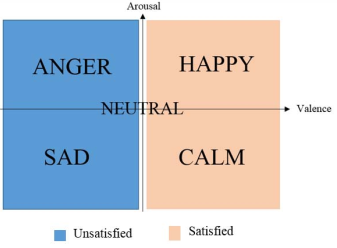
\includegraphics[angle=0, width=0.6\textwidth]{Figures/Satisfaction_from_VA.PNG}
  \caption{Satisfaction inference from VA values}
  \label{fig:SatisfactionFromVA}
  \end{center}
\end{figure}

\citet{Kamaruddin:2016:MeasuringCustomerSatisfaction} realized that using a threshold for defining a 'Neutral' region between Satisfied and Unsatisfied actually performs better in terms of accuracy. They admit that their results are still weak with 40 \% accuracy for measuring satisfaction and 58 \% accuracy for neutral emotion.
% In another approach by \citet{Kamaruddin:2016:MeasuringCustomerSatisfaction}, they built upon the hypothesis that the customer is satisfied if he/she is experiencing happiness and neutral emotion whereas if he/she is experiencing sadness or anger, the customer is dissatisfied. They were using Valence and Arousal values and split them up into four emotional values, including one for neutral emotion. They made use of a threshold to define the neutral emotion class. From these classes they directly inferred whether the customer was satisfied or not. Their accuracy stems from the correct prediction of this classes and is with 39 percent accuracy much better than random guessing with 25 percent.
% \begin{quote}
%     We hypothesize that if the valence value is positive (happiness and calm), the customer is satisfied whereas if the valence value is negative (anger and sadness), the customer is not satisfied. Although such approach is simple, it may give us the better understanding of neutral region threshold so that it can be further used for analysis. \citep{Kamaruddin:2016:MeasuringCustomerSatisfaction}
% \end{quote}
\newline\newline
In a study on ads appreciation conducted by \citet{Poirier:2016:AdsFacialExpression}, the authors measured the effectiveness of ads by analyzing facial expressions. \citet{Poirier:2016:AdsFacialExpression} claims that the emotional journey is the strongest predictor of ad appreciation. Thus, they predict the emotional values for valence and arousal, and look at the curve/profile created by values for valence. The author's assumption seems to be that a certain profile of the valence curve determines whether an ad is successful. This sounds indeed very promising, but also raises the questions whether these ad appreciations in commercial ads also convert into actual positive ratings or even product purchases.
% \citet{Poirier:2016:AdsFacialExpression}, the authors measured the effectiveness of ads through facial expressions.
% \begin{quote}
%     emotional journey, which relates to the positive or negative emotional variation  (valence between -1 and 1 where -1: 100\% negative expression, 1: 100\% positive expression and 0: neutral expression), remains the most powerful predictor of ad appreciation 
% \end{quote}
\newline\newline
\citet{Yeasin:2006:MeasurmentOfInterestFromVideo} present an spatio-temporal approach where they categorize emotions in six classes based on visual data. Subsequently, they use those predicted classes, map them to a 3D affect space and compute the level of interest by calculating: L = W x I.
Hereby, the weight W stands for the relative number of images where most of a motion concentrates. While I represents the intensity of an emotion which is calculated by summing up the values for valence, arousal and stance (3D affect space).
% presents a spatio–temporal approach in recognizing six universal facial expressions from visual data and using them to compute levels of interest. 
% Recognized emotions and used them to calculate a level of interest L, which is calculated as follows: L = W x I. Where I stands for the intensity of an emotion and is calculated through summing up all values from valence, arousal and stance (in a 3D affect space) and mapping these to a range of -5 to +5.
% The weight W is represented by a number in the range of 0 to +1 and measures the relative number of images in a sequence that concentrate most of a motion. The lower the number, the closer the coefficient to 1. \citep{Yeasin:2006:MeasurmentOfInterestFromVideo}



% The FaceReader application \citep{Noldus:2020:Facereader} from Noldus bases their 'Interest' calculation on certain action units instead of recognized emotion values. These action units include:
% \begin{itemize}
%     \item 01 - Inner Brow Raiser
%     \item 02 - Outer Brow Raiser
%     \item 03 - Upper Lid Raiser
%     \item 17 - Chin Raiser
%     \item 20 - Lip Stretcher
%     \item 26 - Jaw Drop
% \end{itemize}
% For the analysis the following time interval is used: Interest - 2 seconds.
